\documentclass[12pt]{article}
\usepackage[top=1in,left=1in, right = 1in, footskip=1in]{geometry}

\usepackage{graphicx}
\usepackage{xspace}
%\usepackage{adjustbox}

\newcommand{\comment}{\showcomment}
%% \newcommand{\comment}{\nocomment}

\newcommand{\showcomment}[3]{\textcolor{#1}{\textbf{[#2: }\textsl{#3}\textbf{]}}}
\newcommand{\nocomment}[3]{}

\newcommand{\jd}[1]{\comment{cyan}{JD}{#1}}
\newcommand{\swp}[1]{\comment{magenta}{SWP}{#1}}
\newcommand{\bmb}[1]{\comment{blue}{BMB}{#1}}
\newcommand{\djde}[1]{\comment{red}{DJDE}{#1}}

\newcommand{\eref}[1]{Eq.~\ref{eq:#1}}
\newcommand{\fref}[1]{Fig.~\ref{fig:#1}}
\newcommand{\Fref}[1]{Fig.~\ref{fig:#1}}
\newcommand{\sref}[1]{Sec.~\ref{#1}}
\newcommand{\frange}[2]{Fig.~\ref{fig:#1}--\ref{fig:#2}}
\newcommand{\tref}[1]{Table~\ref{tab:#1}}
\newcommand{\tlab}[1]{\label{tab:#1}}
\newcommand{\seminar}{SE\mbox{$^m$}I\mbox{$^n$}R}

\usepackage{amsthm}
\usepackage{amsmath}
\usepackage{amssymb}
\usepackage{amsfonts}

\usepackage{lineno}
\linenumbers

\usepackage[pdfencoding=auto, psdextra]{hyperref}

\usepackage{natbib}
\bibliographystyle{chicago}
\date{\today}

\usepackage{xspace}
\newcommand*{\ie}{i.e.\@\xspace}

\usepackage{color}

\newcommand{\Rx}[1]{\ensuremath{{\mathcal R}_{#1}}\xspace} 
\newcommand{\Ro}{\Rx{0}}
\newcommand{\Rc}{\Rx{\mathrm{c}}}
\newcommand{\RR}{\ensuremath{{\mathcal R}}\xspace}
\newcommand{\Rhat}{\ensuremath{{\hat\RR}}}
\newcommand{\Rnaive}{\ensuremath{{\mathcal R}_{\textrm{\tiny naive}}}\xspace}
\newcommand{\tsub}[2]{#1_{{\textrm{\tiny #2}}}}
\newcommand{\dd}[1]{\ensuremath{\, \mathrm{d}#1}}
\newcommand{\dtau}{\dd{\tau}}
\newcommand{\dx}{\dd{x}}
\newcommand{\dsigma}{\dd{\sigma}}

\newcommand{\tstart}{\ensuremath{\tsub{t}{start}}\xspace}
\newcommand{\tend}{\ensuremath{\tsub{t}{end}}\xspace}

\newcommand{\betaeff}{\ensuremath{\tsub{\beta}{eff}}\xspace}
\newcommand{\Keff}{\ensuremath{\tsub{K}{eff}}\xspace}

\newcommand{\pt}{p} %% primary time
\newcommand{\st}{s} %% secondary time

\newcommand{\psize}{{\mathcal P}} %% primary cohort size
\newcommand{\ssize}{{\mathcal S}} %% secondary cohort size

\newcommand{\gtime}{\sigma} %% generation interval
\newcommand{\gdist}{g} %% generation-interval distribution

\newcommand{\geff}{g_{\textrm{eff}}} %% generation-interval distribution

\newcommand{\total}{{\mathcal T}} %% total number of serial intervals

\newcommand{\PP}{{\mathcal P}}
\newcommand{\II}{{\mathcal I}}

\begin{document}

\begin{flushleft}{
	\Large
	\textbf\newline{
		Quantifying the effects of population- and individual-based intervention strategies
	}
}
\newline
\\
Sang Woo Park\textsuperscript{1,*}, Kaiyuan Sun, Benjamin M. Bolker, Bryan T. Grenfell, Jonathan Dushoff, \swp{and maybe others if needed?}
\\
\bigskip
\textbf{1} Department of Ecology and Evolutionary Biology, Princeton University, Princeton, NJ, USA
\\
\bigskip

*Corresponding author: swp2@princeton.edu
\end{flushleft}

\section{Introduction}

\swp{Citations are missing in many places---I can fill them up easily later.}
\swp{Intros are always hard... will eventually re-write a lot of it but wanted to keep something there for now...}

The reproduction number \RR---defined as the average number of secondary cases caused by a primary case---is a key characterstic of an emerging epidemic:
It provides information about whether a disease can invade (i.e., when $\RR > 1$), the level of intervention required to prevent further spread, and the final size of an epidemic.
When an epidemic is ongoing, transmission is affected by changes in population-level immunity and non-pharmaceutical interventions---
these changes in transmission dynamics can be captured by $\RR(t)$, often referred to as the \emph{effective} or \emph{time-dependent} reproduction number.
Interpretation and estimation of $\RR(t)$ has been a key area of research during the current COVID-19 pandemic due to its policy implications.

\swp{This whole paragraph sounds repetitive... just trying to write something quickly to put all the ideas there.}
The main challenge in interpretating $\RR(t)$ can be attribted, in part, to its definition.
Typically, it has been defined as the average number of secondary cases caused by a primary case in a partially susceptible population.
While this definition sounds seemingly intuitive, it is mathematically imprecise.
\swp{I wonder if it's better to leave out two sentences about imprecise-ness of the verbal definition? I sort of like to point it out though.}
Given infection kernel $K(t, \tau)$ representing the rate at which an individual infected $\tau$ time units ago generates secondary cases at time $t$, we can define time-dependent reproduction numbers in two different ways.
First, the instantaneous reproduction number $\RR(t)$---defined as the average number of secondary cases that an individual infected at time $t$ will generate over the course of their infection if conditions at time $t$ were to remain unchanged---corresponds to:
\begin{equation}
\RR(t) = \int K(t, \sigma) \dsigma.
\end{equation}
The instantaneous reproduction number measures conditions at time $t$ and provides a real-time estimate of whether the disease will continue to spread if conditions stay the same;
however, since conditions can continuously change throughout an epidemic, $\RR(t)$ cannot be measured directly (in theory), even if the entire infection process is known, and is difficult to interpret.
On the other hand, we can also define the forward-looking case reproduction number $\Rc(t)$---defined as the average number of secondary cases that an individual infected at time $t$ generated over the course of their infection:
\begin{equation}
\Rc(t) = \int K(t+\dsigma, \dsigma) \dsigma.
\end{equation}
Unlike $\RR(t)$, $\Rc(t)$ can be measured directly (in theory) by taking the average of secondary cases generated by each person and is easy to interpret;
however, $\Rc(t)$ depends on conditions after time $t$ and therefore can only be estimated retrospectively.

\swp{really just throwing out ideas here...}
Estimating $\RR(t)$ adds another layer of challenge: 
It requires knowledge of true incidence of infection $i(t)$ and the generation-interval distribution $g(\tau)$. Definition.
Popularized by Cori et al, an estimator for $\RR(t)$ is given by:
\begin{equation}
\RR(t) = \frac{i(t)}{\int_0^\infty g(\sigma) i(t-\sigma) \dsigma}.
\end{equation}
Current best practices assume that the generation-interval distribution $g(\tau)$ does not vary over time....
This is good for capturing population-based intervention, but not individual-based intervention.
For example, if a strict NPI (e.g., digital contact tracing) that prevents individuals from transmitting after symptom onset, then $g$ would look really different...
Neglecting such changes in $g$ can introduce biases.

In this manuscript, we explore how population- and individual-based interventions can affect population- and individual-level measures of transmission.
Use $r(t)$ as a complementary measure along with $\RR(t)$!!!!!

\section{Mathematical theory}

\subsection{Renewal equation framework}

We begin by introducing the renewal equation framework, which provides a flexible way of modeling the spread of infection and the impact of intervention on the spread.
Throughout this paper, we use $s, t$ to denote calendar time and $\sigma, \tau$ to denote time since infection.
Let $K(t, \tau)$ represent the infection kernel, defined as the rate at which secondary cases are generated at time $t$ by an individual infected $\tau$ time units ago;
the shape of this kernel can depend on internal factors (e.g., variation in infectiousness over the course of infection) or external factors (e.g., susceptible depletion, nonpharmaceutical interventions, changes in behavior).
The integral of $K(t, \tau)$, representing the total infectiousness of an individual infected at time $t$ given conditions at time $t$, corresponds to the instantaneous reproduction number: $\RR(t) = \int K(t, \sigma) \dsigma$.
The kernel, normalized by the total infectiousness, provides information about the time scale of transmission; we refer to this quantity as the instantaneous generation-interval distribution: $g(t, \tau) = K(t, \tau)/\RR(t)$.
Then, incidence at time $t$ caused by a cohort of individuals infected $\tau$ time units ago can be written as the product of the instantaneous reproduction number $\RR(t)$, the instantaneous generation-interval distribution $g(t, \tau)$, and incidence at time $t-\tau$, $i(t-\tau)$:
\begin{equation}
i_{t-\tau}(t) = \RR(t) g(t, \tau) i(t-\tau).
\end{equation}
Integrating across time since infection $\tau$ allows us to express the dynamics of the proportion susceptible $S(t)$ and incidence $i(t)$ in the absence of natural births or deaths as follows: 
\begin{align}
\frac{\mathrm{d}S}{\mathrm{d}t} &= - i(t),\\
i(t) &= \RR(t) \int_0^\infty  g(t, \sigma) i(t-\sigma) \dsigma.
\label{eq:renewal}
\end{align}
For example, in the absence of intervention, the infection kernel $K(t, \tau)$ can be written as a product of proportion susceptible $S(t)$ and the intrinsic kernel $K_0(\tau) = K(0, \tau)$:
\begin{align}
K(t, \tau) &= S(t) K_0(\tau),\\
&= \Ro S(t) g_0(\tau),
\end{align}
where $\Ro$ represents the basic reproduction number, $g_0(\tau)$ represents the intrinsic generation-interval distribution.
This model, also known as renewal equations, generalizes the dynamics of many compartmental models.

While renewal equations are often written in the form of \eref{renewal}, it is also useful to consider the forward-looking renewal equation because neither $\RR(t)$ nor $g(t, \tau)$ are directly measurable (even under the assumption that all infection events can be observed); instead, both quantities rely on the assumption that the condition at time $t$ remains unchanged.
Consider the forward kernel $F_t(\tau)$, which represent the rate at which an individual infected at time $t$ generates a secondary cases $\tau$ time units after infection: 
\begin{equation}
F_t(\tau) = K(t+\tau, \tau) = \RR(t + \tau) g(t+\tau, \tau).
\label{eq:fkernel}
\end{equation}
Unlike the infection kernel $K(t, \tau)$, the forward kernel $F_t(\tau)$ is directly measurable, at least in theory.
The integral of $F(t, \tau)$, representing the total infectiousness of an individual infected at time $t$, corresponds to the case reproduction number: $\Rc(t) = \int F_t(\sigma) \dsigma$;
this quantity can be theoretically measured by taking the average of number of infectees of individuals who were infected at time $t$. 
The kernel, normalized by the total infectiousness, correspond to the forward generation-interval distribution $f_t(\tau) = F_t(\tau)/\Rc(t)$;
this quantity can be theoretically measured by taking the distribution of time between actual infection events (i.e., realized generation intervals, given that the infector was infected at time $t$.
At this point, it is straightforward to see that $F_{t^\ast}(\tau) = K(t^\ast, \tau)$ (and therefore, $\Rc(t^\ast) = \RR(t^\ast)$ and $f_{t^\ast}(\tau) = g(t^\ast,\tau)$) if $K(t, \tau)$ stays invariant after time $t^\ast$ (i.e., $K(t, \tau) = K(t^\ast, \tau)$ for all $t \geq t^\ast$); this hypothetical scenario, in which the condition at time $t^\ast$ remains unchanged after time $t^\ast$, matches the core assumption behind the defition of instantaneous quantities $\RR(t)$ and $g(t, \tau)$.
Then, incidence at time $t$ caused by a cohort of individuals infected $\tau$ time units ago can be written as:
\begin{equation}
i_{t-\tau}(t) = \Rc(t-\tau) f_{t-\tau}(\tau) i(t-\tau).
\end{equation}
Integrating across time since infection $\tau$ gives us the forward renewal equation:
\begin{align}
\frac{\mathrm{d}S}{\mathrm{d}t} &= - i(t),\\
i(t) &= \int_0^\infty \Rc(t-\sigma) f_{t-\sigma}(\sigma) i(t-\sigma) \dsigma.
\label{eq:frenewal}
\end{align}
The forward renewal equation reveals an important insight: Even if the instantaneous generation-interval distribution $g(t, \tau)$ remains invariant across time (i.e., $g(t, \tau) = g(0, \tau)$), changes in $\RR(t)$ causes the forward generation-interval to change (see \eref{fkernel}).
Therefore, renewal equation models that rely on the forward form (\eref{frenewal}) but assume time-invariant $f_t(\tau)$ do not reflect real epidemiological processes and must not be used.

\subsection{Population- and individual-based interventions}

\begin{figure}[!th]
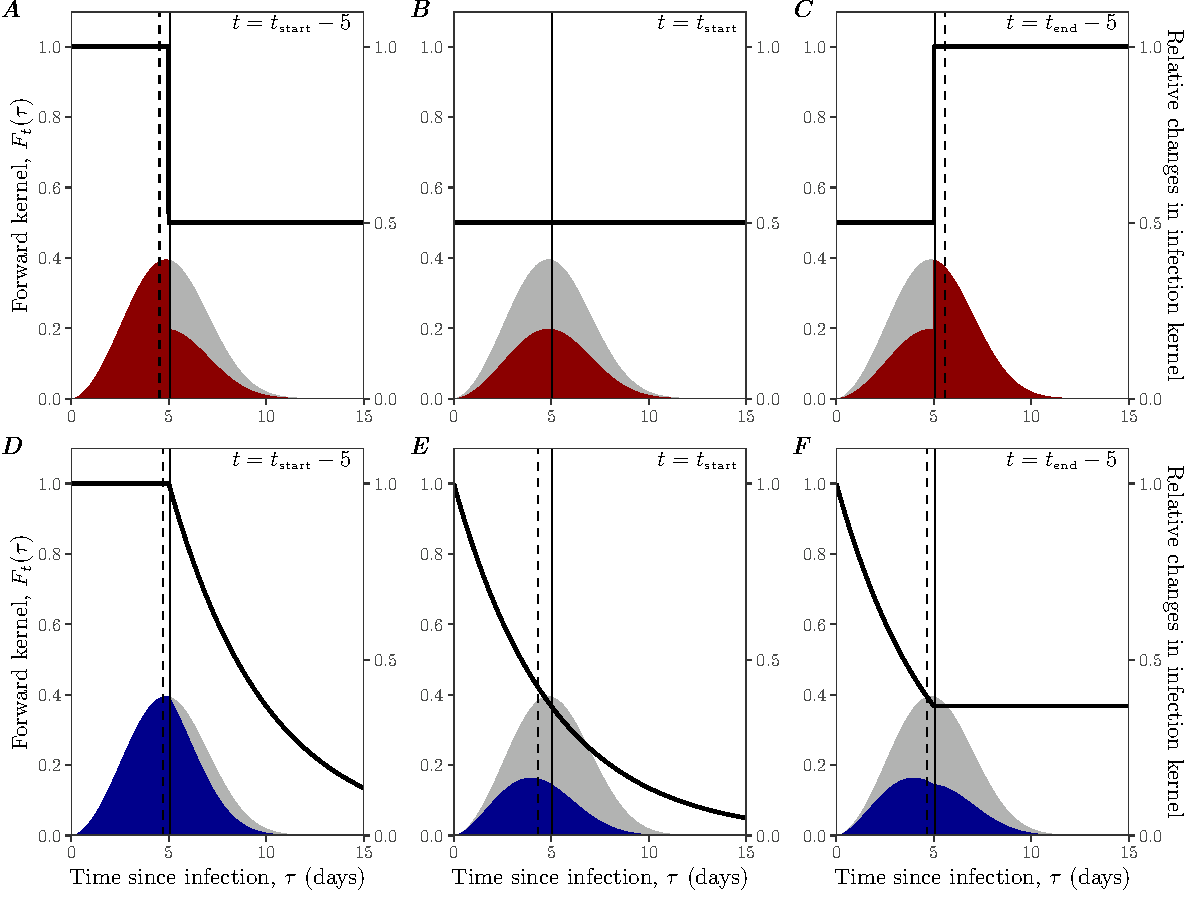
\includegraphics[width=1\textwidth]{pop_ind_compare.pdf}
\caption{
\textbf{The impact of population- and individual-based interventions on forward kernels.}
The impact of constant strength (A--c) and speed (D--F) intervention on forward kernels of individuals infected at different time:
5 days before intervention onset (A, D), during intervention (B, E), and 5 days before intervention offset (C, F).
Gray shaded curves represent the intrinsic kernel $K_0(\tau)$.
Colored curves represent the forward kernel $F_t(\tau)$.
Solid black lines represent relative changes in the kernel: $F_t(\tau)/K_0(\tau)$.
Solid vertical lines the mean intrinsc generation interval.
Dashed vertical lines the mean forward generation interval.
}
\label{fig:indpop}
\end{figure}

To model the impact of intervention during an ongoing epidemic, we first distinguish population-based interventions, which reduces the transmission potential of all (or some fraction of) infected individuals by an equal amount regardless of their time of infection, from individual-based interventions, which target each individual separately and therefore depend on time of infection.
Population-based interventions can be thought of as interventions that reduce the transmission rate and include social distancing, school closures, and vaccination.
Individual-based interventions can be thought of as interventions that reduce the duration of infectious periods and include case isolation and behavioral changes (e.g., symptomatic individuals are more likely to self isolate earlier as awareness increases).

Let $\PP(t)$ represent a population-based intervention that modulates the infection kernel multiplicatively at calendar time $t$ such that $\PP(t)=1$ corresponds to intervention that has no effect and $\PP(t) < 1$ corresponds to intervention that reduces transmission.
Then, the infection kernel under $\PP$ at calendar time $t$ can be written as:
\begin{equation}
K(t, \tau) = \Ro S(t) \PP(t) g_0(\tau).
\end{equation}
Likewise, the forward kernel of an individual infected at time $t$ under $\PP$ can be written as:
\begin{equation}
F_t(\tau) =  \Ro S(t+\tau) \PP(t + \tau) g_0(\tau).
\end{equation}
Here, we see that population-based intervention has same impact on transmission dynamics as susceptible depletion.

For example, a social distancing measure that reduces transmission potential by a factor of $1/\phi$ between time \tstart and \tend can be modeled as:
\begin{equation}
\PP(t) = \begin{cases}
1 & t < \tstart\\
\phi & \tstart \leq t < \tend\\
1 & \tend \leq t
\end{cases}.
\end{equation}
\fref{indpop}A--C illustrates the impact of such intervention on the forward kernel of an individual infected 5 days before $\tstart$, at $\tstart$, and 5 days before $\tend$ (assuming $S(t) \approx 1$).
We present changes in the forward kernel due to its measurability.
Population-based interventions can take effect immediately and sharply reduce transmission (\fref{indpop}A);
likewise, lifting the intervention can, in theory, cause the forward kernel to return back to normal immediately (\fref{indpop}C).
Even though the exact shape of the kernel depends on the time of infection and when the intervention was introduced relative to the infection time, the relative impact of intervention in reducing transmission at any given time (by a factor of $1/\phi$) does not vary across individuals (\fref{indpop}A--C).
Such intervention also has direct effects on realized generation intervals:
implementing (lifting) intervention decreases (increases) future transmission potential and therefore decreases (increases) the mean realized generation interval (\fref{indpop}A,C).
If an individual is infected after \tstart (and much earlier than \tend), this intervention simply reduces the entire kernel by a constant amount and has no effect on realized generation intervals.
This mechanism explains and further generalizes how susceptible depletion leads to contraction of generation intervals in a homogeneously mixing population. 

On the other hand, individual-based intervention $\II(t, \tau)$, such as case isolation, targets each infected individual and therefore depends on calendar time $t$ as well as time since infection $\tau$.
In theory, $\II(t, \tau)$ can capture almost all interventions; here, we use $\II(t, \tau)$ to specifically model interventions that take the following form:
\begin{equation}
\II(t, \tau) = \exp \left(- \int_0^\tau h(t-\tau+\sigma, \sigma) \dsigma \right),
\end{equation}
where $h(t, \tau)$ represents the hazard rate at which an individual infected $\tau$ time units ago will be isolated at calendar time $t$.
Then, $\II(t,\tau)$ can be interpreted as the probability that an individual infected $\tau$ time units ago has not been isolated by calendar time $t$ such that $\II(t, \tau) < 1$ represents reduction in transmission.
In this case, the infection kernel under $\II$ at calendar time $t$ is given by:
\begin{equation}
K(t, \tau) = \Ro S(t) \II(t, \tau) g_0(\tau).
\end{equation}
Likewise, the forward kernel of an individual infected at time $t$ under $\II$ can be written as:
\begin{equation}
F_t(\tau) = \Ro S(t+\tau) \II(t+\tau, \tau) g_0(\tau).
\end{equation}
This intervention is speed-like because its effectiveness depends on how fast we can isolate infected individuals.

For example, given hazard $h(\tau)$ of being isolated, the probability that an individual infected at time $t$ has not been isolated by $\tau$ time units after infection given that the individual-based intervention takes place between time \tstart and \tend depends on the amount of time the individual has been exposed to this intervention.
If the individual was infected before $\tstart$, they will not be isolated until after $\tstart$.
If the individual was infected after $\tend$, they will never be isolated by this intervention.
Therefore, such probability can be modeled as:
\begin{equation}
\II(t+\tau, \tau) = \begin{cases}
1 & t < \tstart-\tau \\
\exp\left(- \int_{\max(0, \tstart - t)}^{\min(\tau, \tend-t)} h(\sigma)\dd{\sigma} \right) & \tstart-\tau \leq t < \tend \\
1 & \tend \leq t
\end{cases}
\end{equation}a
\fref{indpop}D--E illustrates the impact of a single individual-based intervention with constant hazard on the forward kernel of an individual infected 5 days before $\tstart$, at $\tstart$, and 5 days before $\tend$ (assuming $S(t) \approx 1$).
Unlike the population-based intervention, individual-based intervention does not take effect immediately;
that is, the rate at which an infected individual generates a secondary case at time $\tstart$ (e.g., $F_t(\tstart-t)$ in \fref{indpop}D; more generally, $K(\tstart, \tau)$) remains unaffected by the intervention because it takes time to identify and isolate infected individuals.
On the other hand, when the intervention is lifted at $\tend$, the value of the kernel at calendar time $\tend$ ($F_t(\tend-t)$ in \fref{indpop}F; more generally, $K(\tend, \tau)$) remains unchanged because some fraction of infected individuals have already been isolated.
In general, individual-based interventions shorten realized generation intervals because they prevent late transmission (\fref{indpop}D--E).

Finally, given (possibly multiple) population- and individual-based interventions, $P(t)$ and $I(t, \tau)$, the infection kernel can be written as:
\begin{equation}
K(t, \tau) = \Ro S(t) \PP(t) \II(t,\tau) g_0(\tau).
\end{equation}
The corresponding forward kernel can be written as:
\begin{equation}
F_t(\tau) = \Ro S(t+\tau) \PP(t + \tau) \II(t+\tau, \tau) g_0(\tau).
\end{equation}
Therefore, the dynamics of $S(t)$ and $i(t)$ can be now written as:
\begin{equation}
\begin{aligned}
\frac{\mathrm{d}S}{\mathrm{d}t} &= - i(t),\\
i(t) &= \Ro S(t) \PP(t) \int_0^\infty \II(t, \sigma) g_0(\sigma) i(t-\sigma)\dsigma.
\end{aligned}
\end{equation}

\subsection{Quantifying changes in time-dependent reproduction number}

The impact of intervention is often measured by the instantaneous reproduction number $\RR(t)$:
\begin{align}
\RR(t) &= \RR_0 S(t) \PP(t) \int_0^\infty \II(t,\sigma) g_0(\sigma) \dsigma.
\label{eq:rt}
\end{align}
Since $\RR(t)$ measures conditions at time $t$, we expect to observe changes in $\RR(t)$ as soon as intervention is implemented.
Therefore, it provides a real-time measure for whether the disease will continue to spread or not.

Estimating $\RR(t)$ depends on the instantaneous generation-interval distribution $g(t, \tau)$, rather than the intrinsic generation-interval distribution $g_0(\tau)$:
\begin{equation}
g(t, \tau) = \frac{K(t, \tau)}{\RR(t)} = \frac{\II(t,\tau) g_0(\tau)}{\int_0^\infty \II(t,\sigma) g_0(\sigma) \dsigma},
\end{equation}
which can vary across time when individual-based interventions are present.
By rearranging \eref{renewal}, we obtain the following estimator for $\RR(t)$:
\begin{equation}
\RR(t) = \frac{i(t)}{\int_0^\infty g(t, \sigma) i(t-\sigma) \dsigma}.
\end{equation}
While this estimator is similar in form to previously proposed estimators, the main difference is that it allows for the underlying generation-interval distribution to vary to account for individual-based intervention.
In particular, Cori et al have popularized the estimation of $\RR(t)$ via the R package EpiEstim, but it also assumes that the underlying generation-interval distribution does not change over time; 
such method accurately captures changes in $\RR(t)$ under population-based intervention, but not under individual-based intervention.

In general, when both population- and individual-based interventions are present during an ongoing epidemic, the classical estimator that assumes a time-invariant generation-interval distribution measures a slightly different quantity.
Given incidence between time $0$ and $t-\epsilon$ for $\epsilon > 0$, we can calculate the proportional reduction $p(t)$ in true incidence $i(t)$ at time $t$ compared to a counterfactual incidence value that we would observe at time $t$ if all intervention measures were completely removed at time $t$ (including release of isolated individuals):
\begin{align}
p(t) &= \frac{\Ro S(t) \PP(t) \int_0^\infty \II(t, \sigma) g_0(\sigma) i(t-\sigma)\dsigma}{\Ro S(t) \int_0^\infty g_0(\sigma) i(t-\sigma) \dsigma}\\
\end{align}
By substituting true incidence $i(t)$ in the numerator and rearranging, we obtain the classical expression for the estimator for $\RR(t)$---which we refer to as $\tsub{\RR}{prop}(t)$---that depends on the proportion of the susceptible population and proportional reduction in incidence, rather than reduction in infectiousness:
\begin{equation}
\tsub{\RR}{prop}(t) = \Ro S(t) p(t) = \frac{i(t)}{\int_0^\infty g(\sigma) i(t-\sigma) \dsigma}.
\end{equation}
Despite its wide use, this estimator is difficult to interpret in general and does not necessarily serve as a threshold value.

\subsection{Quantifying changes in time-dependent growth rate}

The instantaneous reproduction number $\RR(t)$ measures whether the epidemic will \emph{eventually} grow or decline if current conditions remain unchanged;
counterintuitively, it does not tell us whether the epidemic is growing or not at a given moment.
Interpreting $\RR(t)$ estimates is further impeded by the fact that conditions change during an epidemic.
Instead, if we want to quantify whether incidence is increasing or decreasing, we can simply calculate the epidemic growth rate.
Often growth rates are used measure the initial exponential growth rate; here we generalize the idea by taking the per-capita growth rate:
\begin{equation}
r(t) = \frac{1}{i(t)} \frac{\dd{i(t)}}{\dd{t}}.
\end{equation}
Then, by definition, incidence grows when $r(t) > 0$ (and vice versa).
Although this measure seems tautological, it is the best available measure for capturing whether incidence is growing or not at a given moment.

\subsection{Quantifying changes in the effective generation-interval distribution}

In order to accurately estimate the instantaneous reproduction number, we have to be able to first quantify how the instantaneous generation-interval distribution $g(t, \tau)$ changes across time $t$.
The instantaneous distribution measures the infectiousness of an individual infected $\tau$ time units ago at time $t$ and therefore is different from the distribution of realized generation intervals (i.e., time between actual infection events).
For example, if we were to take all realized generation intervals that end at time $t$ and form a distribution, we obtain what is known as the backward generation-interval distribution, $b_t(\tau)$:
\begin{align}
b_t(\tau) &= \frac{i(t-\tau) K(t,\tau)}{\int_0^\infty i(t-\sigma) K(t,\sigma) \dsigma},\\
&= \frac{i(t-\tau) g(t,\tau)}{\int_0^\infty i(t-\sigma) g(t,\sigma) \dsigma},
\end{align}
which is, in fact, a convolution of the instantaneous generation-interval distribution with previous incidence of infection.

Some studies have suggested substituting the forward distribution $f_t(\tau)$, including the forward serial-interval distribution, instead to estimate $\RR(t)$:
\begin{equation}
\tsub{\RR}{forward}(t) = \frac{i(t)}{\int_0^\infty i(t-\sigma) f_{t-\sigma}(\sigma) \dsigma}.
\end{equation}
However, this choice is also suboptimal.
While both the forward generation-interval distribution $f_{t-\tau}(\tau)$ and the instantaneous generation-interval distribution $g(t, \tau)$ depend on the rate at which secondary cases at time $t$ are generated by a primary case infected at time $t-\tau$, $K(t, \tau)$, they are normalized by different quantities:
\begin{equation}
f_{t-\tau}(\tau) = \frac{K(t,\tau)}{\int_0^\infty K(t-\tau+\sigma,\sigma) \dsigma} \neq \frac{K(t,\tau)}{\int_0^\infty K(t,\sigma) \dsigma} = g(t, \tau).
\end{equation}
The forward distribution $f_{t-\tau}(\tau)$ is normalized by the average number of secondary cases caused by a primary case infected at time $t-\tau$.
On the other hand, the instantaneous distribution $g(t, \tau)$ is normalized by the sum of average number of secondary cases that an individual infected at time $t-x$ will generate at time $t$ (integrated across $x$).

Therefore, even if we can observe all realized generation intervals throughout an epidemic, estimating the instantaneous distribution $g(t, \tau)$ is not trivial.
Even within a homogeneously mixing population, in which the disease is allowed to spread unchecked (and therefore $g(t, \tau) = g_0(\tau)$ for all $t$), aggregating all realized generation intervals underestimates the mean intrisic generation interval due to susceptible depletion.
Either a deconvolution or a novel statistical tool is needed to accurately estimate the instantaneous distribution $g(t, \tau)$.
To our knowledge, no studies have accomplished this yet.

\section{Example: Semi-mechanistic SIR model}

In order to understand how population- and individual-based interventions affect disease spread, we use a semi-mechanistic SIR model to generate synthetic data and compare estimates of $\RR(t)$:
\begin{align}
\frac{\dd{S}}{\dd{t}} &= - \beta(t)S I,\\
\frac{\dd{I}}{\dd{t}} &= \beta(t)S I - \gamma(t) I,\\
\frac{\dd{R}}{\dd{t}} &= \gamma(t) I,
\end{align}
where $S$, $I$, $R$ represent proportion of individuals that are susceptible, infected, and removed (either due to recovery or isolation measures);
$\beta(t)$ represent time-varying transmission rate; and $\gamma(t)$ represent time-varying removal rate.
This model is semi-mechanistic because it allows $\beta$ and $\gamma$ to change over time but their changes are not necessarily driven by any particular mechanism.
In this case, the instantaneous kernel can be written as:
\begin{equation}
K(t, \tau) = \beta(t) S(t) \exp\left(-\int_{t-\tau}^t \gamma(s) \dd{s} \right).
\end{equation}
We see that changes in transmission rate $\beta(t)$ and removal rate $\gamma(t)$ correspond to population- and individual-based intervention.
In particular, abrupt changes in $\gamma(t)$ does not affect the incidence immediately due to delays in isolating individuals.
Finally, the instantaneous reproduction number is given by:
\begin{equation}
\RR(t) = \beta(t) S(t) \int_0^\infty \exp\left(-\int_{t-\tau}^t \gamma(s) \dd{s} \right) \dtau.
\end{equation}
When $\gamma(t) = \gamma(0)$, we obtain a familiar form: $\RR(t) = \Ro S(t)$,
where $\Ro = \beta(0)/\gamma(0)$.

\begin{figure}[!ht]
\includegraphics[width=\textwidth]{figure_beta_gamma.pdf}
\caption{
\textbf{Assumed changes in transmission rate and removal rate.}
The semi-mechanistic SIR model is simulated under six different scenarios.
(A--C) Equivalent population-based intervention scenarios.
Removal rate $\gamma$ is fixed to $1/5\,\textrm{days}^{-1}$ throughout.
(D--F) Equivalent individual-based intervention scenarios.
Transmission rate $\beta$ is fixed to $3/10\,\textrm{days}^{-1}$ throughout.
Each vertical pair of scenarios, referred to as equivalent population- and individual-based intervention scenarios, generates identical incidence curves.
}
\label{fig:assumption}
\end{figure}

Here, we compare six different scenarios, in which intervention is introduced and is later partially/completely lifted (\fref{assumption}).
In the first three scenarios, we consider smooth introduction and lifting of population-based intervention, modeled by changes in $\beta$ while using fixed $\gamma$ (\fref{assumption}A--C).
In the last three scenarios, we consider sudden introduction and lifting of individual-based intervention, modeled by changes in $\gamma$ while using fixed $\beta$ (\fref{assumption}D--F).
We refer to each pair of scenarios as \emph{equivalent} population- and individual-based intervention scenarios because they give identical incidence curves, meaning that changes in $\beta$ and $\gamma$ are jointly unidentifiable (see Methods and Materials).

\begin{figure}
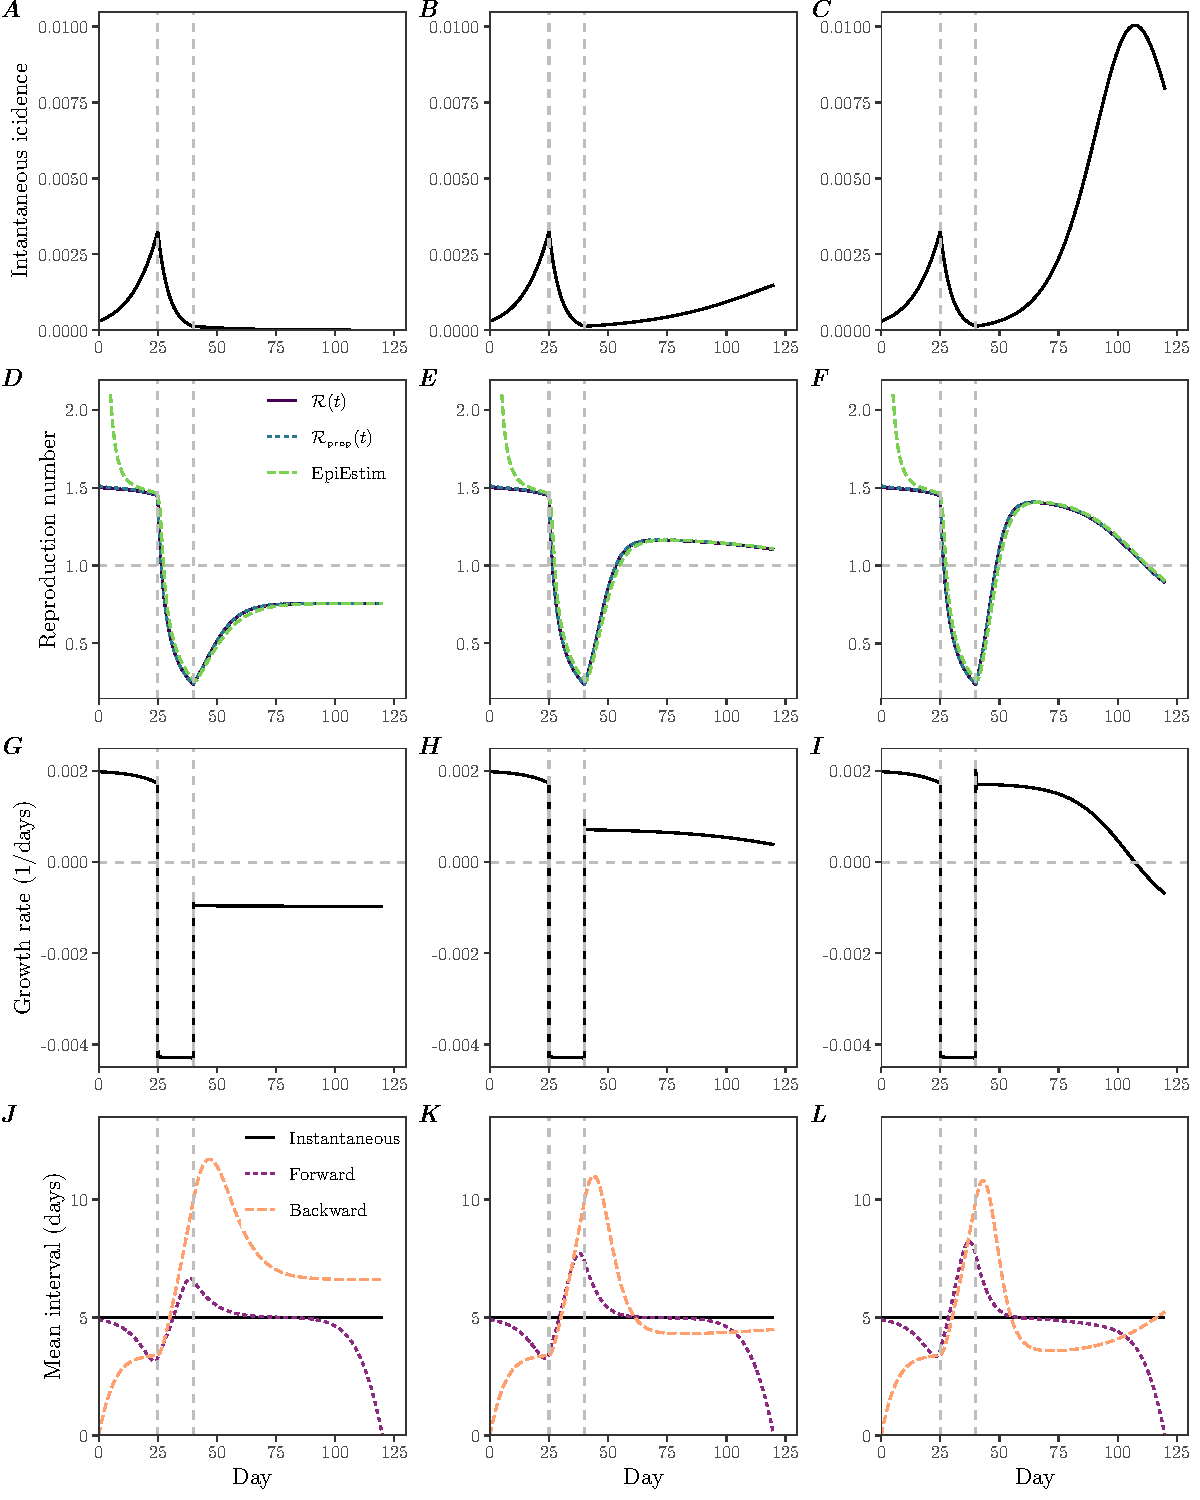
\includegraphics[width=\textwidth]{figure_sir_beta.pdf}
\caption{
\textbf{Epidemiological dynamics of a semi-mechanistic SIR model under equivalent population-based intervention.}
(A--C) Changes in instantaneous incidence over time.
(D--F) Changes in instantaneous reproduction number $\RR(t)$, proportional reproduction number $\tsub{\RR}{prop}(t)$, and estimated $\RR(t)$ using EpiEstim.
(G--I) Changes in instantaneous growth rate.
(J--L) Changes in mean instantaneous, forward, and backward generation intervals.
}
\label{fig:sir_beta}
\end{figure}

Epidemiological dynamics under equivalent population-based intervention are presented in \fref{sir_beta}.
In this case, the instantaneous reproduction number $\RR(t)$ matches the proportional reproduction number $\tsub{\RR}{prop}(t)$ (\fref{sir_beta}D--F).
Likewise, the estimated $\RR(t)$ using \texttt{EpiEstim} matches the true $\RR(t)$;
the initial overestimation of $\RR(t)$ is caused by left-censoring (\fref{sir_beta}D--F).


\begin{figure}
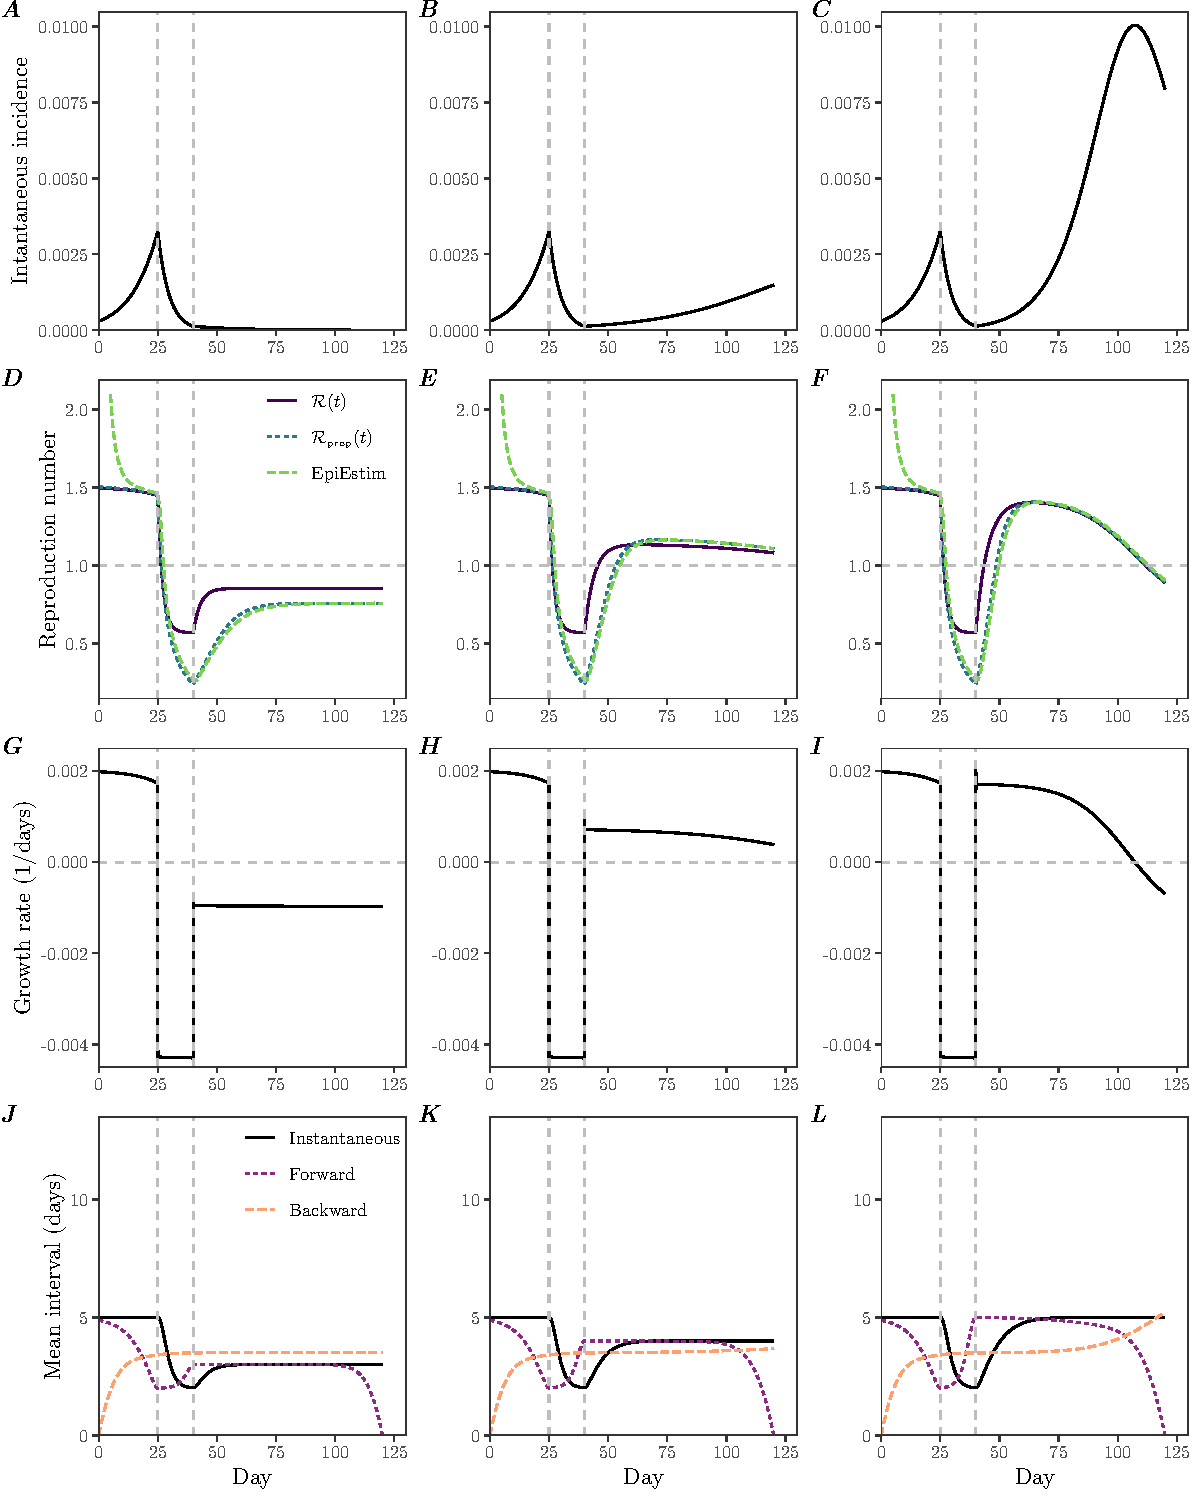
\includegraphics[width=\textwidth]{figure_sir_semi.pdf}
\caption{
\textbf{Epidemiological dynamics of a semi-mechanistic SIR model under equivalent individual-based intervention.}
(A--C) Changes in instantaneous incidence over time.
(D--F) Changes in instantaneous reproduction number $\RR(t)$, proportional reproduction number $\tsub{\RR}{prop}(t)$, and estimated $\RR(t)$ using EpiEstim.
(G--I) Changes in mean instantaneous, forward, and backward generation intervals.
}
\label{fig:sir_semi}
\end{figure}

\section{Discussion}

Speed is cool.

\section{Methods}


Here, we consider a simple scenario in which a flu-like pathogen with $\Ro = 1.5$ invades an immunologically naive population.
In the beginning, the disease spreads without any intervention.
On day 25, an intense case isolation measure is implemented. 
On day 40, the intervention is completely/partially lifted.
This is modeled as follows:
\begin{equation}
\beta(t) = 3/10\,\,\textrm{days}^{-1}, \gamma(t) = \begin{cases}
1/5\,\, \textrm{days}^{-1} & t < 25\\
1/2\,\, \textrm{days}^{-1} & 25 \leq t < 40 \\
\tsub{\gamma}{late} & 40 \leq t
\end{cases},
\end{equation}
where we vary $\tsub{\gamma}{late}$ between $1/3\,\, \textrm{days}^{-1}$ (partial lifting) and $1/5\,\, \textrm{days}^{-1}$ (complete lifting).
Simulations are run for 100 days based on the following initial conditions: $S(0) = 1 - 10^{-3}$, $I(0) = 10^{-3}$, and $R(0) = 0$.

Since we assume that incidence is known exactly until time $t^\ast$, we can, in fact, estimate the transmission rate $\beta^\ast(t)$ (with fixed $\gamma(t)=\gamma(0)$) that gives identical incidence trajectory until time $t^\ast$.
This transmission rate is given by:
\begin{equation}
\beta^\ast(t) = \frac{\tsub{\RR}{prop}(t)\gamma(0)}{S(t)}.
\end{equation}
More generally, given true incidence $i(t)$ and true $\RR(t)$ untile time $t^\ast$, modulated by some combination of population- and individual-based intervention, we can find population intervention $\PP^\ast(t)$ that gives identical incidence until time $t^\ast$:
\begin{equation}
\PP^\ast(t) = \frac{\tsub{\RR}{prop}(t)}{S(t)}.
\end{equation}
We refer to this intervention as the \emph{equivalent} population-based intervention.


\end{document}
